%%%%%%%%%%%%%%%%%%%%%%%%%%%%%%%%%%%%%%%%%
% Short Sectioned Assignment
% LaTeX Template
% Version 1.0 (5/5/12)
%
% This template has been downloaded from:
% http://www.LaTeXTemplates.com
%
% Original author:
% Frits Wenneker (http://www.howtotex.com)
%
% License:
% CC BY-NC-SA 3.0 (http://creativecommons.org/licenses/by-nc-sa/3.0/)
%
%%%%%%%%%%%%%%%%%%%%%%%%%%%%%%%%%%%%%%%%%

%----------------------------------------------------------------------------------------
%	PACKAGES AND OTHER DOCUMENT CONFIGURATIONS
%----------------------------------------------------------------------------------------

\documentclass[paper=a4, fontsize=11pt]{scrartcl} % A4 paper and 11pt font size

\usepackage[margin=0.6in]{geometry}
\usepackage[utf8]{inputenc}
\usepackage[T1]{fontenc} % Use 8-bit encoding that has 256 glyphs
\usepackage{fourier} % Use the Adobe Utopia font for the document - comment this line to return to the LaTeX default
\usepackage[english]{babel} % English language/hyphenation
\usepackage{amsmath,amsfonts,amsthm} % Math packages

\usepackage{lipsum} % Used for inserting dummy 'Lorem ipsum' text into the template
\usepackage{multicol}
\usepackage{sectsty} % Allows customizing section commands
\allsectionsfont{\centering \normalfont\scshape} % Make all sections centered, the default font and small caps

\usepackage{fancyhdr} % Custom headers and footers
\pagestyle{fancyplain} % Makes all pages in the document conform to the custom headers and footers
\fancyhead{} % No page header - if you want one, create it in the same way as the footers below
\fancyfoot[L]{} % Empty left footer
\fancyfoot[C]{} % Empty center footer
\fancyfoot[R]{\thepage} % Page numbering for right footer
\renewcommand{\headrulewidth}{0pt} % Remove header underlines
\renewcommand{\footrulewidth}{0pt} % Remove footer underlines
\setlength{\headheight}{13.6pt} % Customize the height of the header
\usepackage{enumitem}
\setlist{leftmargin=35mm}
\usepackage{graphicx}

\numberwithin{equation}{section} % Number equations within sections (i.e. 1.1, 1.2, 2.1, 2.2 instead of 1, 2, 3, 4)
\numberwithin{figure}{section} % Number figures within sections (i.e. 1.1, 1.2, 2.1, 2.2 instead of 1, 2, 3, 4)
\numberwithin{table}{section} % Number tables within sections (i.e. 1.1, 1.2, 2.1, 2.2 instead of 1, 2, 3, 4)

\setlength\parindent{0pt} % Removes all indentation from paragraphs - comment this line for an assignment with lots of text

%----------------------------------------------------------------------------------------
%	TITLE SECTION
%----------------------------------------------------------------------------------------

\newcommand{\horrule}[1]{\rule{\linewidth}{#1}} % Create horizontal rule command with 1 argument of height

\title{\vspace{-1.5cm}
\normalfont \normalsize 
\textsc{Instituto Superior Técnico\\Universidade de Lisboa} \\ [12pt] % Your university, school and/or department name(s)
\huge Specification of Software 2015/16\\2\textsuperscript{nd} Project Report \\ [5pt]
}

\author{
  Daiane Oliveira\\
  \texttt{ist423160}
  \and
  Tiago Diogo\\
  \texttt{ist173559}
}

\date{\normalsize\today} % Today's date or a custom date

\begin{document}

\maketitle % Print the title

\section{Project Approach}
Given the operations and restrictions presented in the project statement the group decided to use a hierarchical approach, where each machine would be responsible for a specific group of operations and restrictions. This allows the use of a refinement process where each machine considers a single dimension and is then refined and expanded with the operations and restrictions of the next dimension. The used machines are explained in the following section, ordered by the refining sequence (each item refines the previous).

\section{Signatures Modeling and Explanation}


\begin{figure}[h]
  \centering
  \begin{minipage}[b]{0.25\textwidth}
    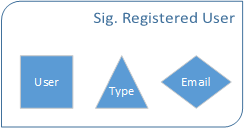
\includegraphics[width=\textwidth]{sig_reg_user.png}
    \caption{Flower one.}
  \end{minipage}
  \hfill
  \begin{minipage}[b]{0.3\textwidth}
    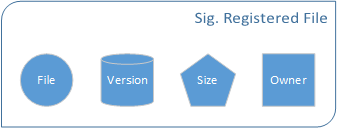
\includegraphics[width=\textwidth]{sig_reg_file.png}
    \caption{Flower two.}
  \end{minipage}
  \hfill
   \begin{minipage}[b]{0.35\textwidth}
    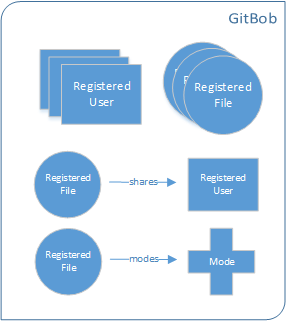
\includegraphics[width=\textwidth]{sig_gitbob.png}
    \caption{Flower one.}
  \end{minipage}
  \hfill
  \begin{minipage}[b]{0.2\textwidth}
    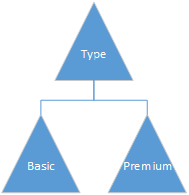
\includegraphics[width=\textwidth]{sig_types.png}
    \caption{Flower two.}
  \end{minipage}
  \hfill
  \begin{minipage}[b]{0.35\textwidth}
    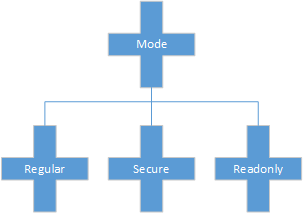
\includegraphics[width=\textwidth]{sig_modes.png}
    \caption{Flower two.}
  \end{minipage}
\end{figure}

\begin{figure}[h]
  \centering
  \begin{minipage}[b]{0.35\textwidth}
    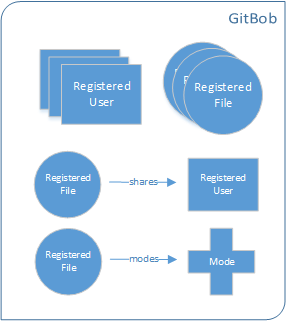
\includegraphics[width=\textwidth]{sig_gitbob.png}
    \caption{Flower one.}
  \end{minipage}
  \hfill
  \begin{minipage}[b]{0.2\textwidth}
    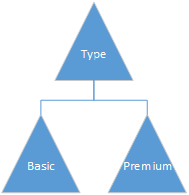
\includegraphics[width=\textwidth]{sig_types.png}
    \caption{Flower two.}
  \end{minipage}
  \hfill
  \begin{minipage}[b]{0.35\textwidth}
    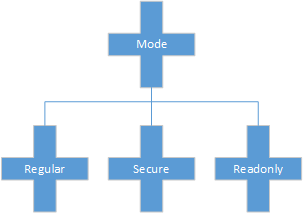
\includegraphics[width=\textwidth]{sig_modes.png}
    \caption{Flower two.}
  \end{minipage}
\end{figure}

\section{Interactive Prover}
The following profs were not automatically proved and required the group intervention
\begin{multicols}{2}
\begin{itemize}
	\item[\textbf{Machine mac\_files}] uploadFile/inv4/INV
	\item[\textbf{Machine mac\_shares}] addFile/inv2/INV
	\item[\textbf{Machine mac\_shares}] downgradeBasic/inv6/INV
	\item[\textbf{Machine mac\_shares}] uploadFile/inv5/INV
	\item[\textbf{Machine mac\_backups}] uploadFileWithBackup/inv2/INV
	\item[\textbf{Machine mac\_backups}] addFile/inv3/INV
	\item[\textbf{Machine mac\_backups}] uploadFileWithBackup/inv2/INV
	\item[]
\end{itemize}
\end{multicols}

\end{document}